\documentclass[12pt]{article}
\usepackage[english]{babel}
\usepackage{url}
\usepackage[utf8]{inputenc}
\usepackage{rotating}
\usepackage{listings}
\usepackage[
backend=biber,
style=numeric,
urldate=long
]{biblatex}
\usepackage{booktabs}
\newcommand{\tabitem}{\makebox[1em][r]{\textbullet~}}
\usepackage{amsmath}
\usepackage{graphicx}
\graphicspath{{images/}}
\usepackage{setspace}
\usepackage{parskip}
\usepackage{fancyhdr}
\usepackage{vmargin}
\usepackage{float}
\usepackage{chngcntr}
\usepackage [autostyle, english = british]{csquotes}
\MakeOuterQuote{"}
\usepackage[format=plain,
            labelfont={bf,it},
            textfont=it,
            justification=centering]{caption}
\usepackage{subcaption}
\counterwithin{figure}{section}
\counterwithin{table}{section}
\setmarginsrb{3 cm}{2.5 cm}{3 cm}{2.5 cm}{1 cm}{1.5 cm}{1 cm}{1.5 cm}

\usepackage{xcolor}

\colorlet{punct}{red!60!black}
\definecolor{background}{HTML}{EEEEEE}
\definecolor{delim}{RGB}{20,105,176}
\colorlet{numb}{magenta!60!black}

\lstdefinelanguage{json}{
    basicstyle=\normalfont\ttfamily,
    numbers=left,
    numberstyle=\scriptsize,
    stepnumber=1,
    numbersep=8pt,
    showstringspaces=false,
    breaklines=true,
    frame=lines,
    backgroundcolor=\color{background},
    literate=
     *{0}{{{\color{numb}0}}}{1}
      {1}{{{\color{numb}1}}}{1}
      {2}{{{\color{numb}2}}}{1}
      {3}{{{\color{numb}3}}}{1}
      {4}{{{\color{numb}4}}}{1}
      {5}{{{\color{numb}5}}}{1}
      {6}{{{\color{numb}6}}}{1}
      {7}{{{\color{numb}7}}}{1}
      {8}{{{\color{numb}8}}}{1}
      {9}{{{\color{numb}9}}}{1}
      {:}{{{\color{punct}{:}}}}{1}
      {,}{{{\color{punct}{,}}}}{1}
      {\{}{{{\color{delim}{\{}}}}{1}
      {\}}{{{\color{delim}{\}}}}}{1}
      {[}{{{\color{delim}{[}}}}{1}
      {]}{{{\color{delim}{]}}}}{1},
}

\title{NewSumm}								% Title
\author{Kunal M L Wagle}								% Author
\date{\today}											% Date


\addbibresource{sample.bib}

\DefineBibliographyStrings{english}{%
urlseen = {Retrieved},
}

\makeatletter
\let\thetitle\@title
\let\theauthor\@author
\let\thedate\@date
\makeatother

\usepackage{imakeidx}
\indexsetup{othercode=\small}
\makeindex[program=makeindex,columns=2,intoc=true,options={-s mystyle.ist}]

\pagestyle{fancy}
\fancyhf{}
\rhead{\theauthor}
\lhead{\thetitle}
\cfoot{\thepage}

\begin{document}

%%%%%%%%%%%%%%%%%%%%%%%%%%%%%%%%%%%%%%%%%%%%%%%%%%%%%%%%%%%%%%%%%%%%%%%%%%%%%%%%%%%%%%%%%

\begin{titlepage}
	\centering
    \vspace*{0.5 cm}
    
\includegraphics[scale = 0.05]{Imperial_College_London_crest.png}\\[1.0 cm]	% University Logo
    \textsc{\LARGE Imperial College London}\\[2.0 cm]	% University Name
	\textsc{\Large C401}\\[0.5 cm]				% Course Code
	\textsc{\large MEng Computing Final Report}\\[0.5 cm]				% Course Name
	\rule{\linewidth}{0.2 mm} \\[0.4 cm]
	{ \huge \bfseries \thetitle \\[0.4cm] \textsc{\large News Aggregator and Summariser}}\\
	\rule{\linewidth}{0.2 mm} \\[1.5 cm]
	
	\begin{minipage}{0.4\textwidth}
		\begin{flushleft} \large
			\emph{Author:}\\
			\theauthor
			\end{flushleft}
			\end{minipage}~
			\begin{minipage}{0.4\textwidth}
			\begin{flushright} \large
			\emph{Supervisor:} \\
			Anandha Gopalan									% Your Student Number
		\end{flushright}
	\end{minipage}\\[2 cm]
	
	{\large \thedate}\\[2 cm]
 
	\vfill
	
\end{titlepage}

%%%%%%%%%%%%%%%%%%%%%%%%%%%%%%%%%%%%%%%%%%%%%%%%%%%%%%%%%%%%%%%%%%%%%%%%%%%%%%%%%%%%%%%%%

\section*{Abstract}
Abstract to be written

\pagebreak

\section*{Acknowledgements}

Acknowledgements to be written

\clearpage

\doublespacing
\tableofcontents
\pagebreak
\listoffigures
\listoftables
\singlespacing
\pagebreak

%%%%%%%%%%%%%%%%%%%%%%%%%%%%%%%%%%%%%%%%%%%%%%%%%%%%%%%%%%%%%%%%%%%%%%%%%%%%%%%%%%%%%%%%%


\section{Introduction}

\subsection{The Problem}

\subsubsection{The Media}

The Fourth Estate is currently enduring one of its toughest passages of time to date. Some of the challenges it faces are familiar, whilst some are new ones that have been created by the onset of the digital age. 

The term "fake news" is now at the forefront of our minds in an atmosphere that is highly charged. The Digital News Report 2016 found that in the United Kingdom only 50\% of readers trust what they say in the news, whilst only 29\% say that they trust journalists (see Figure \ref{TrustInNews}). This statistics appear to be even more dire for the media in the Untied States of America, when the percentages are 33\% for news channels, and 27\% for print journalists.

\begin{figure}[h]
  \centering
    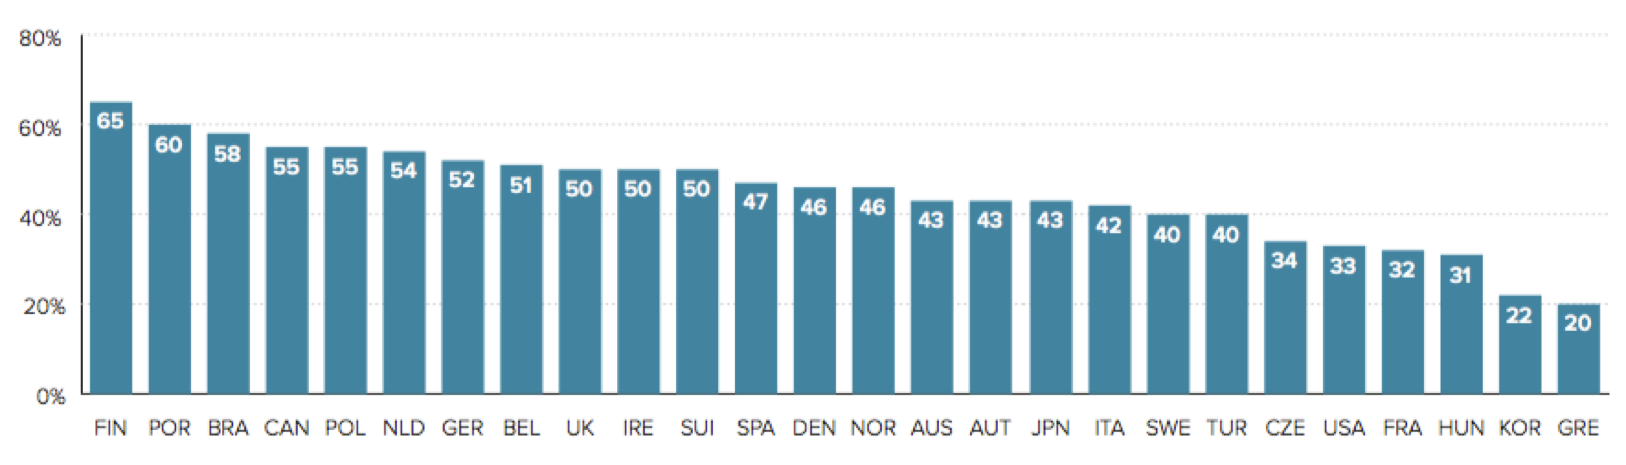
\includegraphics[width=\textwidth]{TrustInNews.png}
   \caption[The Digital News Report 2016 on trust in the news]{Digital News Report findings showed that when it came to trust in the news, in only a few countries was trust as high as 50\% in the accuracy of a piece of news. In countries such as the United States it is far lower.}
   \label{TrustInNews}
\end{figure}

In addition to this, the media have been submerged in a deluge of websites that also claim to disseminate news to readers. In an increasingly digital world, anyone with access to the internet could write a blog about a news story. The popularity of social networks such as Facebook and Twitter also mean that these amateur "journalists" have a platform on which they can compete with professionals from the industry. 

In 2016, the concept of fake news dominated the general election in the United States. Shortly after the country went to the polls, Hillary Clinton's campaign became dogged in rumour after more than a million tweets were sent out about the "pizzagate" scandal. The fake news went both ways. In July 2016, it was reported widely on blogs that Donald Trump had said in an interview with \emph{People} in 1998 that: 

\begin{displayquote}\emph{
"If I were to run, I'd run as a Republican. They're the dumbest group of voters in the country. They believe anything on Fox News. I could lie and they'd still eat it up. I bet my numbers would be terrific."}

\end{displayquote}

The claim was later found to have been fabricated.

Fake news and the people's trust is not the only major issue facing the media at the moment. Another key is sheer volume. Given the abundance of media outlets in the world at the moment, and perhaps more importantly (due to the internet) the accessibility around the globe, there is a lot of competition between outlets. 

\subsubsection{The Consumer}

As a result of a lot of the aforementioned accessibility, consumers also have a challenge in that they can't efficiently read all the news that is out there. If I were to search Google News on the 24th May 2017 for news about Donald Trump, I'd find a story about the President's meeting with the Pope at the Vatican (see Figure \ref{DonaldTrumpPope}). On further inspection, I can see that there are several pages of results about the meeting itself, from dozens of different news sources. A consumer has little to no hope of reading all of these.

\begin{figure}[h]
  \centering
    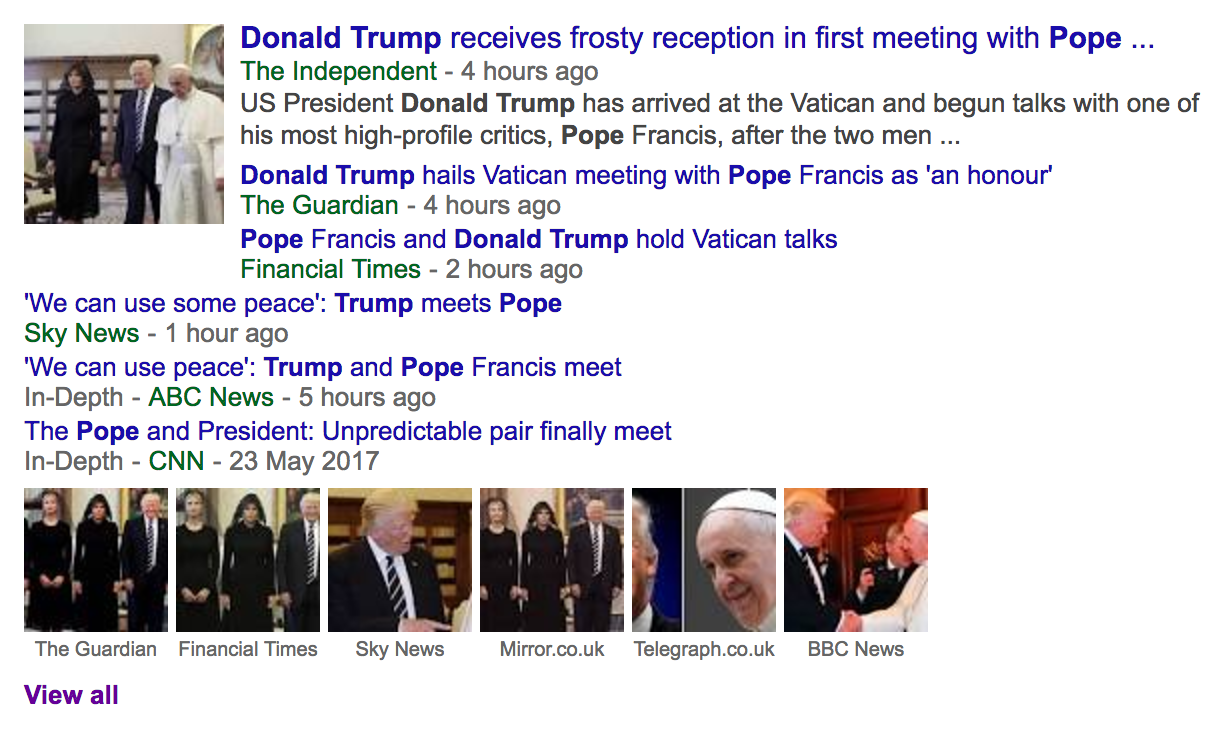
\includegraphics[scale=0.6]{DonaldTrumpPope.png}
   \caption[A Google News Search on 24th May 2017]{A Google News search for stories about President Trump's visit to the Vatican on 24th May 2017}
   \label{DonaldTrumpPope}
\end{figure}

So which news sources should a consumer prioritise? Often, that comes down to political opinion. In fact, the Digital News Report 2016, conducted by the Reuters Institute for the Study of Journalism, says that only 34\% of consumers in the United Kingdom believe that the media is "free from undue political influence". In the United States, which doesn't have a state broadcaster like the United Kingdom does in the BBC, the corresponding statistic is significantly lower at 21\%.

The immediate consequence of statistics like this is that if someone hasn't read all the sources in a piece of news, they are reasonably likely to develop some form of political bias on the issue (perhaps without even realising it). For example, someone who reads about a story in a left-leaning publication such as \emph{The Guardian} may feel differently when compared to someone who reads the corresponding story in a right-leaning publication such as \emph{The Daily Mail}. 

The simple solution to this would be reading the story in as many sources as possible before forming a final opinion. However, as mentioned before, this is just simply not feasible. In July 2016 a study was conducted by the Statistic Brain Research Institute that said that the average attention span of a person is now as low as 8.25 seconds. In addition to this, the Institute's findings also said that the average person only reads 28\% of a webpage of average length (593 words). Another key finding was that users spend only 4.4 seconds to cover each additional 100 words on a webpage. It's simply not possible for every news source to capture a user's attention, especially if they are all broadly covering the same story.

\subsection{News Aggregator and Summariser: A potential solution}

The fundamental aim of my project would be to create a project that directly addresses the consumer's concerns mentioned above, whilst indirectly aiding the concerns of the media.

The project would be a News Aggregator, that would allow users to see the news from multiple mainstream (and therefore "trusted") sources in one place. In addition to this though, the aggregator would also act as a summariser, so that a user doesn't need to read as much as before to gain the same opinion.

However, a key aim has to be to address the issue of there just simply being too much news for someone (who is reading from multiple sources) to take in. To try and achieve this, the News Aggregator will need to identify articles across sources that are about the same topic (for example, Donald Trump's visit to the Vatican), and summarise them. This will mean that a user only has to read a single article to get the full information from multiple sources about a news piece.

In an indirect attempt to allay the concerns of the media and the public about the phenomena that is fake news the News Aggregator will need to find a way to counteract it. One obvious way to do this would be through the limitation of the number of outlets to only those that are "trusted". In addition to this, a clear indication when reading the summary of what facts different outlets all agree on, and what facts they either differ on or omit, will allow the user to easily corroborate parts of the story.

A further secondary aim to this could be to allow a user to customise their summary, taking in information from the outlets of their choice (from the original "trusted" list). The advantage to this would potentially be that if a user decides that too many issues from one source are uncorroborated, they can remove them, and see only information from the other sources that have written about a topic. The disadvantage to this could be that if a user dismisses an entire section of the political spectrum as fake continuously, they'll still pick up a political bias on the facts of the topic. Although, it could be said that the Digital News Report 2016 findings suggest that this is a feature that won't be used much. One of the more interesting findings in the report was that more than 60\% (in the United Kingdom) were concerned about the potential impact of personalising their news feeds. They felt that it could lead to both "missing information" and "missing challenging viewpoints". 

\end{document}